% Modelo de monografia em LaTeX da UECE baseado no template disponibilizado
% por Rudy Matela em http://www.larces.uece.br/~rudy/pub/modelo_monografia/

\documentclass[pnumabnt,normaltoc,capchap,floatnumber=continuous]{abnt}		
\usepackage[bibjustif,abnt-etal-cite=3,abnt-full-initials=yes]{abntcite}
\usepackage{modelo/tex/uece}
\usepackage[toc,page]{modelo/tex/appendix}
\usepackage[portuguese,brazilian,portuges]{babel}
\usepackage[utf8]{inputenc}
\usepackage{abnt-alf}
\usepackage{graphicx}
\usepackage{multicol}
\usepackage{listings}
\usepackage{booktabs}
\usepackage{amsmath}
\usepackage{amsthm}
\usepackage{eucal}
\usepackage{amssymb}
\usepackage{mathrsfs}
\bibliographystyle{abnt-alf}

\usepackage[T1]{fontenc}
\errorstopmode

\hyphenation{com-pu-ta-ção}
\hyphenation{com-bi-na-tó-ria}

\setcounter{secnumdepth}{3}
\setcounter{tocdepth}{3}

\setlength{\topmargin}{-0.3in}

\local{Fortaleza - Ceará}
\cidade{Fortaleza}
\data{2010}

% Informações institucionais
\centro{Centro de Ciências e Tecnologia}
\curso{Graduação em Ciência da Computação}
\cursosimples{Ciência da Computação}
\instituicao{Universidade Estadual do Ceará}

% Descrição para folha de rosto
\comentario{
Monografia apresentada no Curso de \ABNTcursodata\ do \ABNTcentrodata\ da
\ABNTinstituicaodata, como requisito parcial para obtenção do grau de Bacharel
em \UECEcursosimples. 
}

% Descrição um pouco simplificada (removendo o nome do curso ¬¬)
\comentariosimplificado{
Monografia apresentada no Curso de \ABNTcursodata\ do \ABNTcentrodata\ da
\ABNTinstituicaodata, como requisito parcial para obtenção do grau de Bacharel.
}



% Informações gerais do documento
\autor{Sérgio Luis Olinda Braga Correia}
\autorr{Correia, Sérgio Luis Olinda Braga}
\titulo{O protocolo de roteamento bioinspirado Ant-DYMO em VANETs}
\orientador{Joaquim Celestino Júnior}

% essas informacoes do codigo CIP você consegue indo na biblioteca central
\codigocip{C824p}{CDD:001.6}


% Epígrafe: citação e autor (OPCIONAL)
\epigrafe{``So many beautiful women and so little time.''}
\autorepigrafe{John Barrymore}


% Membros da comissão avaliadora
\bancaum{Prof. Dr. \ABNTorientadordata\ -- UECE\\(Orientador)}
\bancadois{Prof. Dr. Gustavo Augusto de Lima Campos -- UECE} 
\bancatres{Prof. Dr. Jorge Luiz de Castro e Silva -- UECE}

% data de aprovação
\dataaprovacao{15/04/2010}

% Palavras chave
\pcs{VANET}{Roteamento}{ACO}{NS-2}{SUMO}
\kws{VANET}{Routing}{ACO}{NS-2}{SUMO}

\begin{document}

% início do documento. lembrando que o documento é
% composto de elementos pre-textuais e pos-textuais,
% alem do texto propriamente dito
%
% sao OBRIGATÓRIOS os seguintes elementos pre-textuais:
% - capa
% - folha de rosto
% - folha de catalogação (CIP)
% - termo de aprovação
% - resumo
% - abstract
%
% sao OPCIONAIS os seguintes:
% - dedicatória
% - agradecimentos
% - epígrafe (citacao)
% - listas de figuras, tabelas, siglas, etc

\capa
\folhaderosto
\makecippage
\termodeaprovacao

% AGRADECIMENTOS - opcional
\pretextualchapter{Agradecimentos}

\noindent
À minha família, pelo incentivo e apoio nos momentos difíceis. 

\noindent
Aos amigos que conheci na UECE ao longo destes anos, pela ajuda e
amizade. Em especial, aos colegas Filipe Maciel, Jeandro Mesquita, Rudy Matela,
Sérgio Vieira, Pablo Ximenes e demais computeiros.

\noindent
Ao professor Joaquim Celestino Júnior pela orientação e oportunidades de
iniciação à pesquisa.

\noindent
Aos professores Gustavo Campos e Everardo Maia pelas discussões
produtivas que contribuíram para este trabalho. 

\noindent
À maioria dos professores que tive durante este curso de Ciência da
Computação da UECE, por sua dedicação, comprometimento e compreensão. 

\noindent
Aos professores que não estão incluídos no grupo anterior, por mostrar
como não se deve fazer as coisas, caso um dia eu me torne um professor.

\noindent
A todas as pessoas que passaram pela minha vida e contribuíram para a
construção de quem sou hoje.

\pagebreak

\makeepigrafe

% sumario
\renewcommand{\contentsname}{SUMÁRIO}
\tableofcontents

% caso haja lista de figuras
\listadefiguras

% caso haja lista de tabelas
\listadetabelas

% caso haja lista de siglas
%   exemplo de sigla:
%   \sigla{UECE}{Universidade Estadual do Ceará}
\listadesiglas

% espaço de um e meio
\onehalfspace


% RESUMO - obrigatorio
\begin{resumo}
\noindent
\sigla{VANETs}{Vehicular Ad hoc NETworks} (\textit{Vehicular Ad hoc NETworks})
são um tipo especial de rede móvel \textit{ad hoc} (\sigla{MANET}{\textit{Mobile ad
hoc NETwork}}, \textit{Mobile ad hoc NETwork}) formada por veículos entre si, e
entre veículos e dispositivos que fazem parte da infraestrutura de ruas e
rodovias. Apesar de compartilharem várias características com as MANETs
tradicionais, as VANETs apresentam algumas diferenças significativas, como por
exemplo o movimento do nós, aleatórios nas MANETs, mas relativamente ordenado
nas VANETs, já que os veículos têm de obedecer as chamadas regras de trânsito.
Neste trabalho, o protocolo de roteamento bioinspirado Ant-DYMO é simulado em
um cenário veicular e tem seu desempenho comparado com o do protocolo DYMO.
Além disso, é proposta uma modificação simples no mecanismo de criação de
formigas do protocolo bioinspirado original, com o objetivo de verificar
possíveis melhoras no desempenho geral do algoritmo, quando levando em
consideração algumas das características próprias das redes veiculares, como a
informação da vizinhança de veículos.
% deixe essa linha em branco

\vspace{1cm}
\noindent
\palavraschave
\end{resumo}
\pagebreak

% ABSTRACT - obrigatorio
\begin{abstract}
\noindent
VANETs (Vehicular Ad hoc NETworks) are a special type of the Mobile Ad hoc
NETworks (MANETs), made by vechicles communicating between themselves as well as
by vechicles communicating with devices located at the margins of roads and
highways. Despite sharing many characteristics with the traditional
MANETs, VANETs present some siginificant differences. For instance, the
nodes movement, completely random in MANETs, but relatively ordered in the
VANETs, since the nodes -- the vehicles -- are supposed to obey a set of
transit rules. In this work, the bio-inspired routing protocol Ant-DYMO is
evaluated in a VANET scenario and has its performance compared with the DYMO
protocol. Furthermore, a simple modification is proposed in the bio-inspired
mechanisms of Ant-DYMO. The objective is to verify a possible improvement in
the overall performance of the algorithm when taking into account some
characteristics inherent to the vehicular networks, such as neighboring
vehicle information.
% deixe essa linha em branco

\vspace{1cm}
\noindent
\keywords
\end{abstract}
\pagebreak

% agora adicione os capítulos
\chapter{As redes veiculares}
\label{chapter:vanets}

\section{O que são redes veiculares?}
As VANETs (\textit{Vehicular Ad hoc NETworks}) são um tipo especial de rede
móvel ad-hoc (\nomenclature{MANET}{\textit{Mobile Ad hoc NETwork}}, \textit{Mobile Ad
hoc NETwork}) formada entre veículos (\nomenclature{V2V}{\textit{Vehicle-to-vechicle}} -
Figura \ref{fig:v2v}) e entre veículos e dispositivos de infraestrutura
(\nomenclature{V2I}{\textit{Vehicle-to-infrastructure}} - Figura \ref{fig:v2i}). Os
dispositivos instalados nos veículos são conhecidos por \textit{unidades de
bordo} (\nomenclature{OBU}{\textit{On-board unit}}, \textit{On-board unit}) e os que
ficam ao longo da estrada são denominados por \textit{unidades de acostamento}
(\nomenclature{RSU}{\textit{Road-side unit}}, \textit{Road-side unit}).

\begin{figure}[htbp]
\centering
 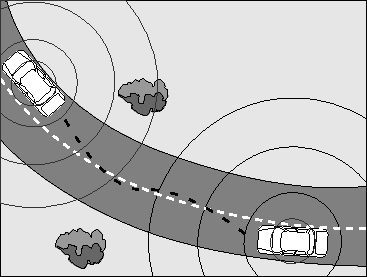
\includegraphics[width=.35\textwidth]{chapters/fig/v2v.pdf}
\caption{Comunicação veículo-veículo}
\label{fig:v2v}
\end{figure}

\begin{figure}[htbp]
\centering
 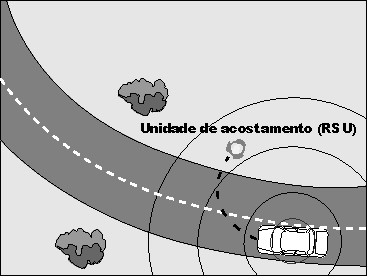
\includegraphics[width=.35\textwidth]{chapters/fig/v2i.pdf}
\caption{Comunicação veículo-infraestrutura}
\label{fig:v2i}
\end{figure}

Na comunicação V2V, cada OBU funciona em modo \textit{ad hoc} podendo encaminhar
mensagens através de múltiplos saltos. Porém, neste modo, a conectividade da
rede é altamente dependente da densidade de veículos na vizinhança e do padrão
de mobilidade.

No modo V2I, a conectividade da VANET pode aumentar através de comunicação com
outras redes. Contudo, o custo de implantação aumenta bastante, pois há
necessidade de termos RSUs espalhados pelas estradas e rodovias.

Apesar de possuírem várias características semelhantes às das MANETs
tradicionais, as VANETs apresentam algumas diferenças significativas, por
exemplo, nas MANETs os nós podem movimentar-se aleatoriamente, já nas VANETS,
sua movimentação é relativamente ordenada, já que os veículos têm de obedecer
regras de trânsito e seguirem um caminho definido.

As redes veiculares têm por objetivo fornecer diversas aplicações aos seus
usuários, tanto no que diz respeito à segurança quanto ao entretenimento. Tal
sistema de aplicações é conhecido por Sistema de Transporte Inteligente
(\nomenclature{ITS}{\textit{Intelligent Transportation System}}, \textit{Intelligent
Transportation System}). Pode-se citar alguns exemplos de aplicações
VANETs, como as aplicações de auxílio à mudança de faixa, aplicações de
descoberta de melhor rota a um determinado destino, aplicações de divulgação de
avisos de segurança, e acesso à internet, dentre outros \cite{li2007routing}.

Grandes são os desafios para a efetiva utilização das VANETs em um cenário
real. Por conta de suas características únicas como alta velocidade de
movimentação e densidade altamente dinâmica, grande parte dos protocolos
utilizados nas MANETs não são adequados \cite{taha2007vanet}. Além destes 
desafios, outros de grande importância referem-se ao baixo tempo de conexão 
entre veículos e a alta possibilidade de perda de conexão durante a 
transmissão de dados.

As redes veiculares são promissoras, visto que permitem oferecer diversos
serviços de comunicação aos motoristas e passageiros, e isso pode ser percebido
com o atual envolvimento da comunidade científica e da indústria automotiva.
Além destes, órgãos governamentais dos Estados Unidos, União Européia e Japão e
organizações de padronização demonstram crescente interesse nessa nova
modalidade de redes de comunicação. O governo americano aprovou em $2003$ um
sistema de comunicação de curta distância, o DSRC (Dedicated
Short-Range Communications) voltado principalmente para as redes veiculares;
a União Européia, por meio de fabricantes de automóveis e peças, iniciou o
consórcio \nomenclature{C2C-CC}{\textit{Car-to-Car Communication Consortium}}
(\textit{Car-to-Car Communication Consortium}) e o IEEE está trabalhando na
família de padrões IEEE 1609, voltados à tecnologia
\nomenclature{WAVE}{\textit{Wireless Access in Vehicular Environments}}
(\textit{Wireless Access in Vehicular Environments}).

Este capítulo vai discutir as redes veiculares, passando pela arquitetura,
cenários onde as redes veiculares poderiam ser utilizadas, características,
aplicações em potencial e desafios técnicos.

\section{Padrões e Arquitetura DSRC/WAVE}
Em $1991$, o congresso americano aprovou a Lei da Eficiência do Transporte
Intermodal de Superfície (\textit{Intermodal Surface Transportation
Efficiency Act}), que resultou na criação da primeira geração dos sistemas de
transportes inteligentes (\nomenclature{ITS}{\textit{Intelligent Transportation
System}}, \textit{Intelligent Transportation
System}). O objetivo principal do programa ITS era o aumento da segurança nos
transportes, que seria obtido com o uso de tecnologia na infraestrutura dos
sistemas de transporte. A primeira geração do DSRC operava em $915$ MHz e tinha
uma taxa de transmissão de $0,5$ Mb/s. Esta tecnologia foi utilizada
principalmente por veículos comerciais e nos sistemas de pagamento de pedágios
(\textit{toll collection}), e teve sucesso limitado. Um exemplo de aplicação
dessa primeira geração do DSRC é o sistema de pedágio eletrônico
\textit{EZPass}. A segunda geração do DSRC iniciou em 1997, quando a sociedade
ITS América requisitou ao FCC a alocação de 75 MHz adicionais. Em 1999 o FCC
alocou 75 MHz na faixa de banda de $5,9$ GHz para esta segunda geração.

Desde a alocação da largura de banda, os organismos de padronização vêm
trabalhando nos detalhes de implementação do DSRC $5,9$ GHz. O objetivo
principal destes esforços é permitir que os motoristas recebam informações
atuais do ambiente que os cerca, como tráfego, informações sobre os veículos
vizinhos, como suas posições e velocidades, o que possibilitaria reduzir
o número de acidentes.

\subsection{Características do DSRC 5,9 GHz}
O DSRC é uma espécie de complemento das comunicações celulares, provendo altas
taxas de transferência em circustâncias onde minimizar a latência nos
\textit{links} de comunicação e isolar pequenas zonas de
comunicação é importante \cite{guo2006vehicular}. O DSRC é também conhecido
como WAVE, e um grupo de trabalho do IEEE está atualmente trabalhando na
padronização das camadas física (PHY) e de acesso ao meio (MAC) sob o padrão
IEEE 802.11p, que no momento da escrita deste trabalho encontra-se ainda em
estado de \textit{draft} \cite{80211p}. A razão pela qual as
camadas PHY e MAC estão sendo desenvolvidas sob a família de padrões 802.11 é a
garantia da sua estabilidade com o passar do tempo. Uma das causas do sucesso
limitado que a primeira geração DSRC 915 MHz experimentou foi devido a poucas
implementações seguirem o padrão fielmente, optando geralmente por soluções
propretárias. Essa foi a maior motivação de a segunda geração DSRC $5,9$ GHz
ser um padrão aberto.

O novo DSRC $5,9$ GHz é um avanço em relação ao seu predecessor 915 MHz em
vários aspectos, como a própria largura de banda, que é maior no novo DSRC. No
DSRC 5,9 GHz, o espectro é composto de sete canais de 10 MHz cada, com um canal
reservado para controle e os outros seis funcionando como canais de serviço. O
antigo DSRC 915 MHz suportava apenas um ou dois canais. A taxa de transmissão,
de apenas $0,5$ Mb/s na primeira geração, agora varia entre $6$ Mb/s e $27$
Mb/s. Em algumas circunstâncias, dois canais de serviço podem ser combinados
para formar um canal único de 20 MHz, possibilitando atingir uma taxa de
transferência de $54$ Mb/s. A única interferência na banda de $5,9$ GHz vem de
radares militares e \textit{uplink} de satélites -- ambos esparsamente
localizados --, ao passo que, a banda de 902--928 MHz é mais sucetível a 
interferências, seja devido a telefones 900 MHz, dispositivos de identificação 
automática instalados nas ferrovias (\textit{AEI readers}) e outros dispositivos 
de observação meteorológica, como radares que detectam a velocidade e direção 
dos ventos.  A tabela \ref{tab:dsrccomparison}, retirada de \cite{guo2006vehicular}, 
mostra as diferenças entre as tecnologias DSRC de primeira e segunda geração.

\begin{table}[htbp]
		\centering
		\begin{tabular}{l l l}
		\toprule
		& 902--928 MHz & 5850--5925 MHz\\
		\midrule
		Espectro & $12$ MHz & $75$ MHz\\
		Taxa de dados  & $0,5$ Mb/s & $6$ Mb/s -- $27$ Mb/s \\
		Potencial de interferência & alto & baixo \\
		Cobertura & uma zona de comunicação & zonas de comunicação sobrepostas\\
		Alcance máximo & $300$ pés ($91,4$ metros) & $1000$ metros\\
		Separação mínima & 1500 pés ($457,2$ metros) & 50 pés ($15,2$ metros)\\
		Canais & 1 a 2 canais & 7 canais\\
		\bottomrule
		\end{tabular}
\caption{Comparação entre as tecnologias DSRC}
 \label{tab:dsrccomparison}
\end{table}

Como dito anteriormente, o espectro DSRC é dividido em sete canais 
de $10$ MHz (Figura \ref{fig:dsrc}) e cada canal é utilizado por um
tipo de aplicação.

\begin{figure}[htbp]
\centering
 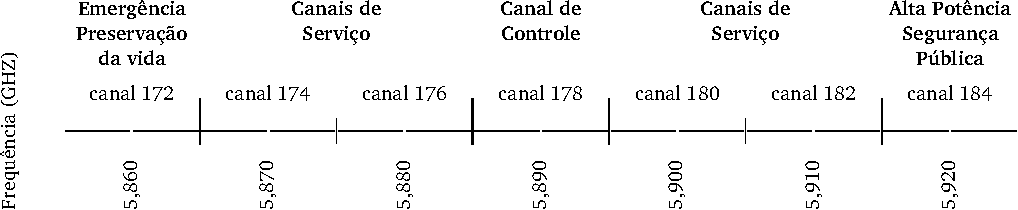
\includegraphics[width=.95\textwidth]{chapters/fig/dsrc.pdf}
\caption{Espectro DSRC}
\label{fig:dsrc}
\end{figure}

O canal de controle (CCH), $178$, é utilizado para comunicação de segurança e
os canais $172$ e $184$ são utilizados para futuras aplicações de emergência e
preservação da vida e para alta potência e segurança pública, respectivamente.
Já os canais de serviço $174$, $176$, $180$ e $182$ são utilizados para
aplicações de segurança ou por outros tipos de aplicação.


\section{Características das redes veiculares}

As redes veiculares apresentam características únicas que as tornam
radicalmente diferentes \cite{blum2004challenges} de outras MANETs, e  
tais características influenciam diretamente o desenvolvimento de 
seus protocolos e serviços. Por conta disto, muitos dos protocolos 
desenvolvidos para MANETs não funcionam adequadamente quando utilizados 
em VANETs. 

Basicamente, uma VANET possui as seguintes características:
\begin{enumerate}
  \item[$\bullet$] alta velocidade dos nós da rede;
  \item[$\bullet$] fornecimento de energia virtualmente ilimitado;
  \item[$\bullet$] alta capacidade computacional;
  \item[$\bullet$] mobilidade previsível.
\end{enumerate}

A combinação destas características resulta em uma topologia altamente 
mutável que é frequentemente fragmentada e possui um pequeno diâmetro 
efetivo da rede, também possui limitada redundância e diversos problemas 
de segurança \cite{raya2006securing, dotzer2006privacy, golle2004detecting}.

Quanto maior a mobilidade dos veículos maior é a mudança da topologia, 
e essa mudança frequente resulta em curtos períodos de conectividade
entre os nós, que podem mover-se a velocidades superiores a 200 km/h, 
por exemplo. Uma possível solução para aumentar o tempo de conectividade 
entre veículos seria aumentar a potência de transmissão, mas isso também 
diminui o \textit{throughput} da rede \cite{khorashadi2007impact,chen2007impact}. 
Por outro lado, como a trajetória dos veículos é restrigida pelo traçado 
da estrada, sua posição futura pode ser considerada previsível, e isto pode
ser utilizado como métrica de um protocolo de roteamento fazendo com que
sejam escolhidas rotas que possuam maior tempo de vida previsto.

A potência de transmissão dos OBUs geralmente não é uma restrição significativa
como ocorre em algumas redes de sensores sem fio. Um veículo consegue fornecer
alimentação contínua para os dispositivos de comunicação.

Outra característica interessante é a capacidade das redes veiculares 
serem formadas por um número potencialmente grande de participantes -- 
podendo se estender por toda uma estrada --, ao contrário da maioria 
das redes \textit{ad hoc} estudadas na literatura, que normalmente assumem um 
tamanho limitado da rede. 

\section{Aplicações potenciais}
As aplicações imaginadas para as redes veiculares variam desde aplicações que
visam à segurança do veículo ou do motorista a aplicações voltadas ao
entretenimento dos passageiros, fazendo uso de uma gama de tecnologias
diferentes.

As ideias primárias das redes veiculares incluem aplicações de segurança para
os motoristas e passageiros, provendo segurança e oferecendo ferramentas para a
decisão do melhor caminho em uma estrada. Tais aplicações, portanto, pretendem
minimizar os acidentes e melhorar as condições de tráfego, oferecendo informações 
úteis aos motoristas e passageiros, como avisos de colisões, notificações
sobre as condições da estrada e visões \textit{in-place} do tráfego
\cite{moustafa2009vehicular}. Para que as aplicações de segurança possam ser 
utilizadas, é necessário que os veículos compartilhem informações precisas de 
posicionamento. As aplicações potenciais desta categoria são as seguintes:

\begin{enumerate}
 \item[$\bullet$] Aplicações cooperativas de alerta de colisão -- auxiliam o
 motorista a evitar choques com a traseira de outros veículos.
 \item[$\bullet$] Aplicações de colisão iminente -- geram informações aos
 mecanismos de segurança (\textit{air bags} ou cintos de segurança, por exemplo)
 para tentar diminuir os danos causados pelos acidentes.
 \item[$\bullet$] Aplicações que alertam sobre locais perigosos -- compartilham
 informações sobre estradas escorregadias, buracos ou outras situações de risco.
\end{enumerate}

A pesquisa atual em redes veiculares foca também nas aplicações de conforto,
que oferecem -- aos motoristas e passageiros --, serviços tais como a
conectividade com a \textit{Internet}, explorando uma infraestrutura disponível
sob demanda, sistemas de pedágio automático, e uma variedade de serviços
multimídia. Além disso, outras redes de comunicação, tais como 2-3G,
\nomenclature{WLANs}{\textit{Wireless Local Area Networks}}
\nomenclature{IEEE}{\textit{Institute of Electric and Electronic Engineers}}
802.11a/b/g/p e \nomenclature{WiMAX}{\textit{Worldwide Interoperability for Microwave
Access}}, podem ser exploradas para fornecer as aplicações de conforto e
entretenimento. As aplicações potencias desta categoria são as seguintes:

\begin{enumerate}
 \item[$\bullet$] Aplicações de acesso à \textit{Internet}.
 \item[$\bullet$] Aplicações de notificação de pontos de interesse -- permite
 obter informações sobre as empresas locais, atrações turísticas ou outras.
 \item[$\bullet$] Aplicações de diagnóstico -- permitem que uma estação de
 serviço avalie o estado de um veículo sem fazer uma inspeção física.
\end{enumerate}
 
\section{Principais desafios}
As características inerentes às redes veiculares criam alguns desafios para a
comunicação veicular, que podem dificultar uma futura utilização dessas redes no
mundo real. Para que este tipo de rede esteja realmente pronta para o
\textit{deployment} e para oferecer serviços úteis aos passageiros e
motoristas, dois problemas importantes precisam ser resolvidos: a
escalabilidade e a interoperabilidade. Os protocolos e mecanismos utilizados
devem escaláveis a numerosos veículos e interoperáveis com diferentes
tecnologias sem fio.

O ambiente de operação de uma VANET é extremamente dinâmico e necessita de
configurações extremas. A velocidade relativa entre veículos pode superar os
$200$ km/h em rodovias e possuir baixa densidade de veículos. Logo em seguida, a
diferença de velocidade pode baixar substancialmente ao mesmo tempo em que a
densidade aumenta consideravelmente.

A rápida mudança de topologia força o desenvolvimento de padrões e aplicações
bastante restritos ao tempo de funcionamento e, por conta de sua fragmentação
frequente, setores da rede podem não se comunicar com outros veículos
localizados em regiões próximas.

Os cenários VANETs são diferentes dos cenários MANETs clássicos. No cenário
urbano, dependendo da situação ou do horário, a densidade da rede pode variar
bastante, passando frequentemente de baixa para alta densidade.




% bibliografia
\bibliography{references}

% caso haja apêndices, use apendice antes de inserir
% as secoes
\apendice
% adicione os apendices, caso existam
\chapter{Modelo de desvanecimento de \textit{Nakagami}}
\label{apendice:nakagami}

O modelo de propagação de \textit{Nakagami} é usado para modelar um
canal de rádio com desvanecimento. Comparado a outros modelos existentes, como
o \textit{Shadowing} e o \textit{Two-Ray Ground}, o modelo de \textit{Nakagami}
apresenta mais parâmetros de configuração que permitem uma representação mais
fiel de um canal de comunicação \textit{wireless}. Ele é capaz de modelar
desde canais totalmente livres de desvanecimento a canais com desvanecimento
moderado, como uma \textit{highway}, por exemplo.

A distribuição de \textit{Nakagami} \cite{nakagami1957m} é definida pela
seguinte função de densidade de probabilidade:

\begin{displaymath}
f(x) =
\frac{2m^{m}x^{2m-1}}{\Gamma(m)\Omega^{m}}\exp\Bigg[-\frac{mx^{2}}{\Omega}\Bigg],
\ x \geq 0,\ \Omega > 0,\ m \geq \frac{1}{2}
\end{displaymath}

A função de densidade de probabilidade correspondente à potência -- quadrado da
amplitude do sinal -- em uma dada distância pode ser obtida por uma mudança de
variáveis e é dada por uma distribuição gama da seguinte forma:

\begin{displaymath}
p(x) =
\Bigg(\frac{m}{\Omega}\Bigg)^{m}\frac{x^{m-1}}{\Gamma(m)}\exp\Bigg[-\frac{mx}{\Omega}\Bigg],
\ x \geq 0
\end{displaymath}

$\Omega$ é o valor esperado da distribuição e pode ser interpretado como a
potência média recebida. $m$ é o parâmetro de desvanecimento.

Os valores dos parâmetros $m$ e $\Omega$ são funções da distância, e o modelo
de \textit{Nakagami} é então definido por duas funções: $\Omega(d)$ e $m(d)$.

\begin{itemize}
  \item\ A distribuição de \textit{Rayleigh} \cite{papoulis2002probability}
  é um caso especial da de \textit{Nakagami}, onde $m(d) = 1$ para qualquer $d$.
  \item\ Valores maiores de $m$ resultam em desvanecimento menos acentuado.
\end{itemize}



% fim :)

\end{document}

